% Created 2023-01-22 Sun 14:31
% Intended LaTeX compiler: xelatex
\documentclass[12pt,twoside,landscape]{extarticle}
\usepackage{graphicx}
\usepackage{longtable}
\usepackage{wrapfig}
\usepackage{rotating}
\usepackage[normalem]{ulem}
\usepackage{amsmath}
\usepackage{amssymb}
\usepackage{capt-of}
\usepackage{hyperref}
\usepackage{subcaption}
\usepackage[newfloat]{minted}
\usepackage{color}
\usepackage{listings}
\usepackage[top=5mm,bottom=5mm,right=5mm,left=5mm,landscape]{geometry}
\usepackage{multicol}
\usepackage{enumitem}
\usepackage{fancyhdr}
\usepackage{caption}
\usepackage{algorithm}
\usepackage{algpseudocode}
\usepackage{float}
\setlist{noitemsep, topsep=0pt}
\setlength{\parindent}{0pt}
\setlength{\columnseprule}{0.2pt}
\definecolor{mygreen}{rgb}{0,0.6,0}
\definecolor{mygray}{rgb}{0.5,0.5,0.5}
\definecolor{mymauve}{rgb}{0.58,0,0.82}
\lstset{ backgroundcolor=\color{white}, basicstyle=\footnotesize, breaklines=true, captionpos=b, commentstyle=\color{mygreen}, escapeinside={\%*}{*)},keywordstyle=\color{blue}, stringstyle=\color{mymauve},}
\author{Olivier Lischer}
\date{\today}
\title{ComBau Exam Summary}
\hypersetup{
 pdfauthor={Olivier Lischer},
 pdftitle={ComBau Exam Summary},
 pdfkeywords={},
 pdfsubject={},
 pdfcreator={Emacs 27.2 (Org mode 9.5.5)}, 
 pdflang={English}}
\begin{document}

\begin{multicols}{4}

\section{General}
\label{sec:org7b5a2bf}
\subparagraph{Chomsky Hierarchy} \
\label{sec:org0b228d1}
The Chomsky Hierarchy describes what is required to read and understand a specific language.
Lexer, Parser and Semantic Checker reads the Language while the \href{../../../roam/20211109182310-deterministic_finite_automaton.org}{DEA}, Push down Automata and Bounded Turing Machine runs the application.

{
\begin{center}
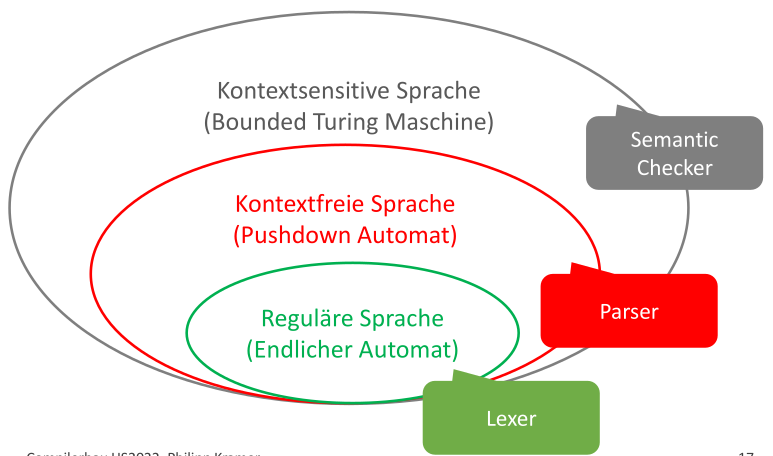
\includegraphics[width=.9\linewidth]{img/chomsky_hierarchie.png}
\end{center}
\captionof{figure}{Chomsky Hierarchy}\label{fig:chomsky-hierarchy}
}

\section{Parser}
\label{sec:org1cd8a81}
\subparagraph{Parser Categories} \
\label{sec:org9a60e97}
\begin{itemize}
\item first letter
\begin{description}
\item[{L}] read from left to right
\item[{R}] read from right to left
\end{description}
\item second letter
\begin{description}
\item[{L}] Left-most expansion (top-down parser)
\item[{R}] right-most reduction (bottom-up parser)
\end{description}
\item number in parentheses
\begin{itemize}
\item number of symbols look ahead
\end{itemize}
\end{itemize}

{
\begin{center}
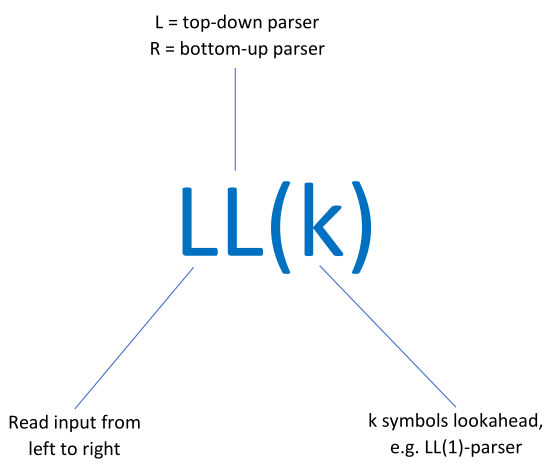
\includegraphics[width=.9\linewidth]{img/parser_notation.png}
\end{center}
\captionof{figure}{Parser notation}\label{fig:parser-notation}
}

\section{Checker}
\label{sec:org8e99352}
\subparagraph{Symbol Table} \
\label{sec:orgc98b086}
The Symbol Table is a data structure produced by the \href{../../../roam/20221228115353-what_is_a_semantic_checker.org}{Semantic Checker}.
The Symbol table is used to manage all declaration in a program source code.

The symbol table contains a mapping from \emph{Symbol} to the \emph{AST} node (\texttt{node = symbolTable.getDeclarationNode(symbol);})


{
\begin{center}
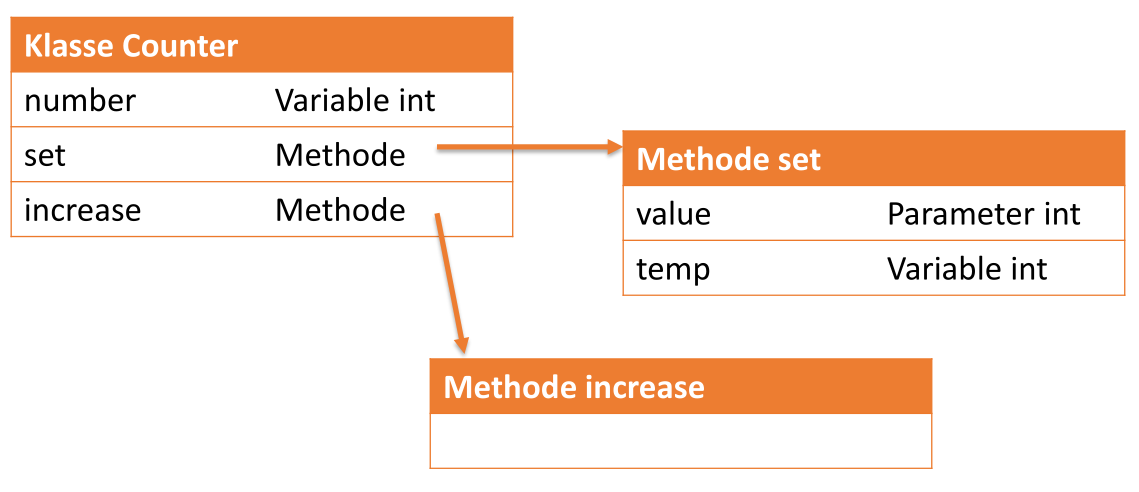
\includegraphics[width=.9\linewidth]{img/symbol_table_example.png}
\end{center}
\captionof{figure}{Example Structure for a Symbol Table}\label{fig:example-structure-for-a-symbol-table}
}
\section{VM}
\label{sec:org64ebcae}
\subparagraph{Ancestor Table} \
\label{sec:org470da50}
The ancestor table is used to check if a class inherits from another in constant time.
In \autoref{fig:ancestor-table-example} you see an example how such an ancestor table is constructed.
The last element in the table for each class is the reference to itself.
However, this only works for \textbf{Single-Inheritance}.

In languages like \href{../../../roam/20201116150053-java.org}{Java} you don't have to allocate memory for the \texttt{object} class, because every class inherits from it (in the ancestor table this would be -1).

{
\begin{center}
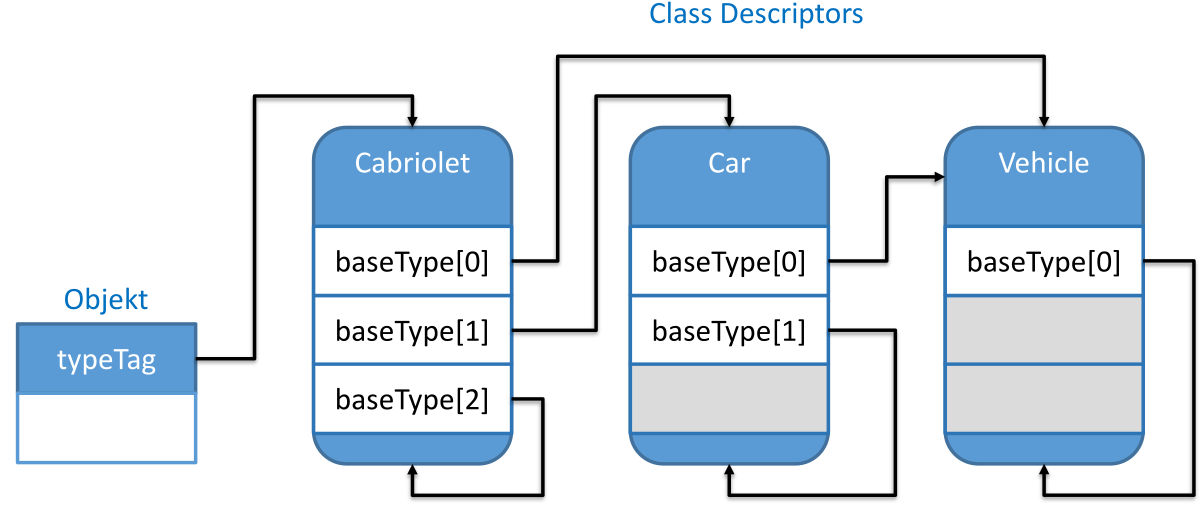
\includegraphics[width=.9\linewidth]{img/ancestor_table.png}
\end{center}
\captionof{figure}{Ancestor Table Example}\label{fig:ancestor-table-example}
}

\subparagraph{Type Cast / Checking} \
\label{sec:orga5c8e26}
You have a target type (you want to cast into this type) and a source type (you want to cast from this type).

\begin{enumerate}
\item Get the ancestor level from the target type (for example 0). Call the level \texttt{x}
\item Check in the ancestor table of the source type if the ancestor at level \texttt{x} is the same as the target class
\end{enumerate}


\begin{lstlisting}[language=java,label= ,caption= ,captionpos=b,numbers=none]
private boolean typeTest(Pointer instance, ClassDescriptor targetType) {
    ClassDescriptor sourceType = heap.getDescriptor(instance);
    if (sourceType == targetType) {
	return true;
    }
    var level = targetClass.getAncestorLevel();

    if (sourceClass.getAncestorTable().length > level) {
	return sourceClass.getAncestorTable()[level] == targetClass;
    } else {
	return false;
    }
}
\end{lstlisting}

\subparagraph{Virtual Table} \
\label{sec:orgb4781b1}
Each type has a Virtual Method Table (vtable).
The vtable describes which virtual method should be called when dynamic dispatch is performed. 
In a \href{../../../roam/20221230173400-what_is_a_virtual_machine.org}{VM} the vtable often points not directly to the function but to the method descriptor.

However, this only works with \textbf{Single-Inheritance}.

{
\begin{center}
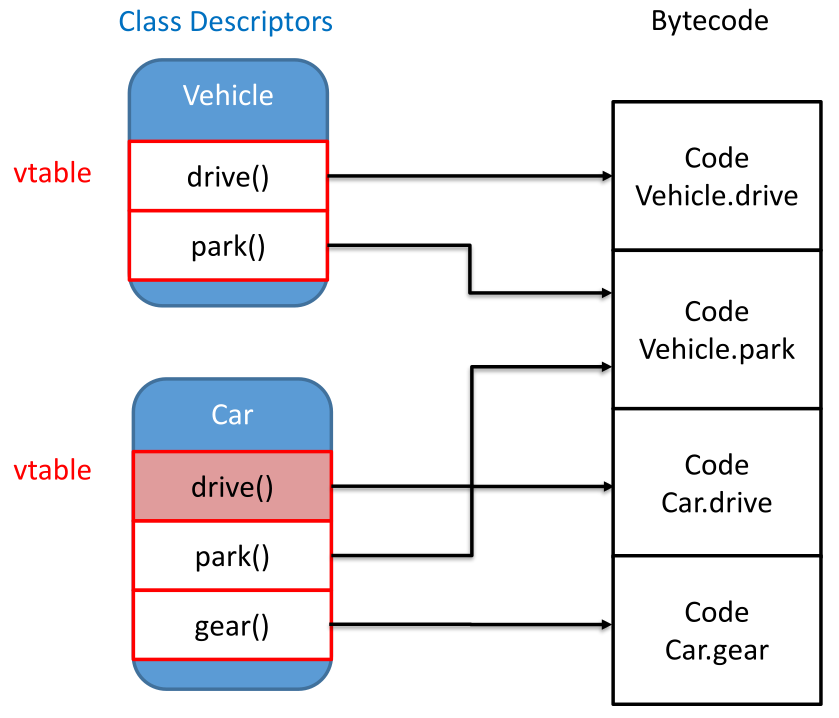
\includegraphics[width=.9\linewidth]{img/vtable_example.png}
\end{center}
\captionof{figure}{VTable example}\label{fig:vtable-example}
}

\subparagraph{Interface Support} \
\label{sec:org2c81d77}
To implement dynamic polymorphism using Interfaces you can't use the same approach as using a \href{../../../roam/20221230181314-what_is_the_virtual_method_table.org}{vtable} in inheritance.
Because you would end up with inconsistent numbering (see \autoref{fig:bad-interface-implementation-attempt}).

{
\begin{center}
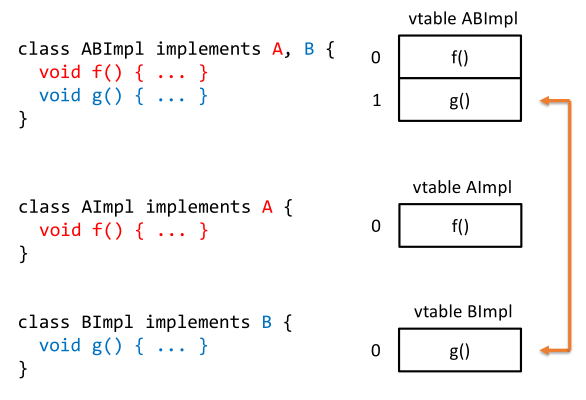
\includegraphics[width=.9\linewidth]{img/interface_bad_attempt.png}
\end{center}
\captionof{figure}{Bad Interface Implementation Attempt}\label{fig:bad-interface-implementation-attempt}
}

To support interfaces you have to globally numbering all interfaces.
For each class you also have to generate an interface table (itable).
This table contains only the implemented interfaces at the same index as they are globally numbered (see \autoref{fig:interface-support}).

{
\begin{center}
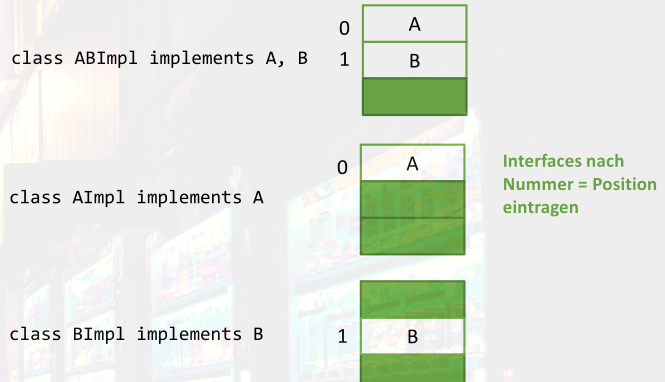
\includegraphics[width=.9\linewidth]{img/interface_support_2.png}
\end{center}
\captionof{figure}{Interface Support}\label{fig:interface-support}
}

To safe memory you can generate a single itable with different offsets.

{
\begin{center}
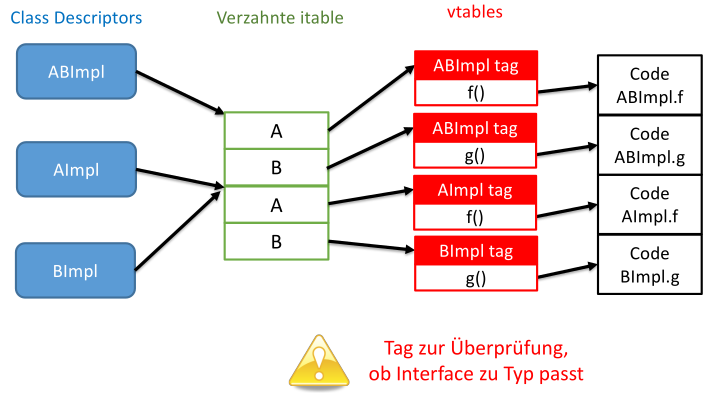
\includegraphics[width=.9\linewidth]{img/total_interface_support.png}
\end{center}
\captionof{figure}{Total Interface Support}\label{fig:total-interface-support}
}

\subparagraph{Allocation Record} \
\label{sec:org8dd2ec7}
The JIT Compiler has to track the usage of the processor registers.
For this you could use the Allocation Record.
The allocation record contains:
\begin{itemize}
\item a list of registers for parameters
\item a list of registers for local variables
\item a set of registers for not used / free registers (missing in \autoref{fig:allocation-record-load-variable})
\item and a linked list / stack for the \href{../../../roam/20221230171752-what_is_a_evaluation_stack.org}{Evaluation Stack}
\end{itemize}


{
\begin{center}
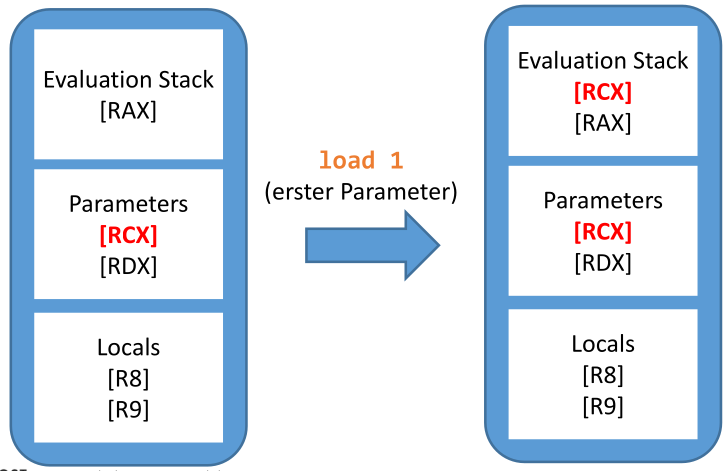
\includegraphics[width=.9\linewidth]{img/allocation_record_load_var.png}
\end{center}
\captionof{figure}{Allocation Record: Load Variable}\label{fig:allocation-record-load-variable}
}
\section{GC}
\label{sec:orgedae212}
\subparagraph{Generational GC} \
\label{sec:orga213972}
A Generational GC is an incremental GC because it often does not clean up the whole heap but in generations.
For example, you have 3 generations as describe in \autoref{tbl:example-for-generations}

\begin{table}[htbp]
\caption{\label{tbl:example-for-generations}Example for generations}
\centering
\begin{tabular}{llll}
age & generation & GC frequency & GC break\\[0pt]
\hline
new & G0 & high & short\\[0pt]
middle & G1 & middle & middle\\[0pt]
old & G2 & low & long\\[0pt]
\end{tabular}
\end{table}

If you want to clean up \emph{Gn} you must extend your root set with all references from the latter generations which are pointing into \emph{Gn}.
If you want to clean up \emph{Gn} you also have to clean up all previous generations.

{
\begin{center}
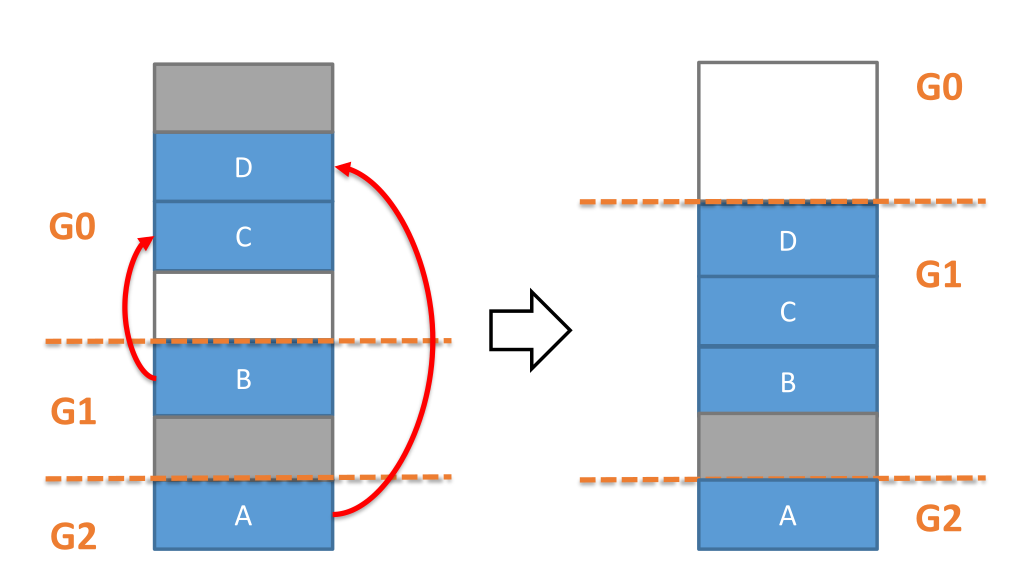
\includegraphics[width=.9\linewidth]{img/gc_of_g0.png}
\end{center}
\captionof{figure}{GC of G0}\label{fig:gc-of-g0}
}

\subparagraph{Resurrection} \
\label{sec:orgfa7f20d}
A finalizer can revive objects (no garbage anymore).
This can happen not only for the current object but also for other objects.


{
\begin{center}
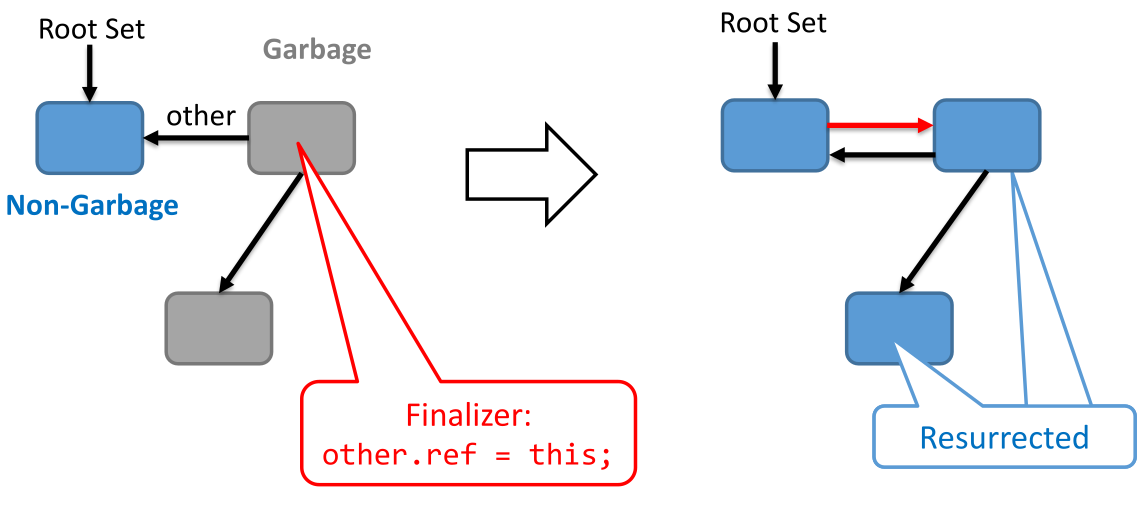
\includegraphics[width=.9\linewidth]{img/resurrection_example.png}
\end{center}
\captionof{figure}{Resurrection Example}\label{fig:resurrection-example}
}


\end{multicols}
\end{document}